% Created by tikzDevice version 0.12.6 on 2024-06-11 16:07:52
% !TEX encoding = UTF-8 Unicode
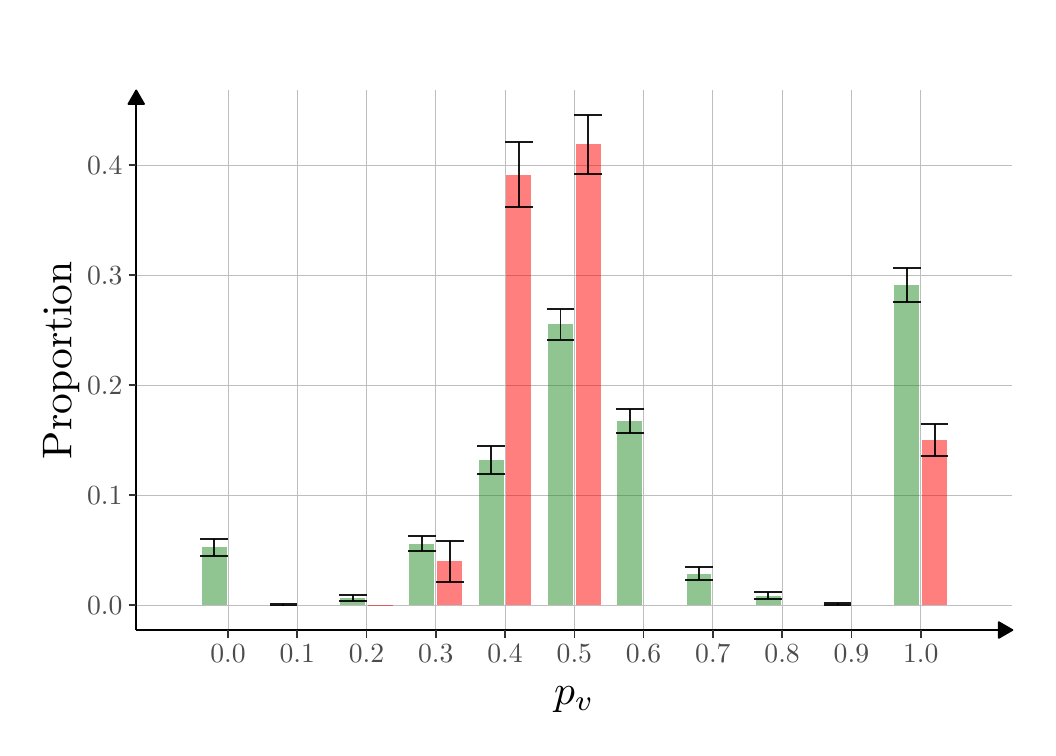
\begin{tikzpicture}[x=1pt,y=1pt]
\definecolor{fillColor}{RGB}{255,255,255}
\path[use as bounding box,fill=fillColor,fill opacity=0.00] (0,0) rectangle (361.35,252.94);
\begin{scope}
\path[clip] (  0.00,  0.00) rectangle (361.35,252.94);
\definecolor{drawColor}{RGB}{255,255,255}
\definecolor{fillColor}{RGB}{255,255,255}

\path[draw=drawColor,line width= 0.6pt,line join=round,line cap=round,fill=fillColor] (  0.00,  0.00) rectangle (361.35,252.94);
\end{scope}
\begin{scope}
\path[clip] ( 39.22, 35.28) rectangle (355.85,230.29);
\definecolor{fillColor}{RGB}{255,255,255}

\path[fill=fillColor] ( 39.22, 35.28) rectangle (355.85,230.29);
\definecolor{drawColor}{RGB}{255,255,255}

\path[draw=drawColor,line width= 0.3pt,line join=round] ( 39.22, 64.15) --
	(355.85, 64.15);

\path[draw=drawColor,line width= 0.3pt,line join=round] ( 39.22,103.90) --
	(355.85,103.90);

\path[draw=drawColor,line width= 0.3pt,line join=round] ( 39.22,143.64) --
	(355.85,143.64);

\path[draw=drawColor,line width= 0.3pt,line join=round] ( 39.22,183.39) --
	(355.85,183.39);

\path[draw=drawColor,line width= 0.3pt,line join=round] ( 39.22,223.14) --
	(355.85,223.14);

\path[draw=drawColor,line width= 0.3pt,line join=round] ( 47.36, 35.28) --
	( 47.36,230.29);

\path[draw=drawColor,line width= 0.3pt,line join=round] ( 59.87, 35.28) --
	( 59.87,230.29);

\path[draw=drawColor,line width= 0.3pt,line join=round] ( 84.90, 35.28) --
	( 84.90,230.29);

\path[draw=drawColor,line width= 0.3pt,line join=round] (109.93, 35.28) --
	(109.93,230.29);

\path[draw=drawColor,line width= 0.3pt,line join=round] (134.96, 35.28) --
	(134.96,230.29);

\path[draw=drawColor,line width= 0.3pt,line join=round] (159.99, 35.28) --
	(159.99,230.29);

\path[draw=drawColor,line width= 0.3pt,line join=round] (185.02, 35.28) --
	(185.02,230.29);

\path[draw=drawColor,line width= 0.3pt,line join=round] (210.05, 35.28) --
	(210.05,230.29);

\path[draw=drawColor,line width= 0.3pt,line join=round] (235.08, 35.28) --
	(235.08,230.29);

\path[draw=drawColor,line width= 0.3pt,line join=round] (260.11, 35.28) --
	(260.11,230.29);

\path[draw=drawColor,line width= 0.3pt,line join=round] (285.14, 35.28) --
	(285.14,230.29);

\path[draw=drawColor,line width= 0.3pt,line join=round] (310.17, 35.28) --
	(310.17,230.29);

\path[draw=drawColor,line width= 0.3pt,line join=round] (335.20, 35.28) --
	(335.20,230.29);

\path[draw=drawColor,line width= 0.3pt,line join=round] (347.72, 35.28) --
	(347.72,230.29);
\definecolor{drawColor}{RGB}{190,190,190}

\path[draw=drawColor,line width= 0.3pt,line join=round] ( 39.22, 44.28) --
	(355.85, 44.28);

\path[draw=drawColor,line width= 0.3pt,line join=round] ( 39.22, 84.02) --
	(355.85, 84.02);

\path[draw=drawColor,line width= 0.3pt,line join=round] ( 39.22,123.77) --
	(355.85,123.77);

\path[draw=drawColor,line width= 0.3pt,line join=round] ( 39.22,163.52) --
	(355.85,163.52);

\path[draw=drawColor,line width= 0.3pt,line join=round] ( 39.22,203.26) --
	(355.85,203.26);

\path[draw=drawColor,line width= 0.3pt,line join=round] ( 72.39, 35.28) --
	( 72.39,230.29);

\path[draw=drawColor,line width= 0.3pt,line join=round] ( 97.42, 35.28) --
	( 97.42,230.29);

\path[draw=drawColor,line width= 0.3pt,line join=round] (122.45, 35.28) --
	(122.45,230.29);

\path[draw=drawColor,line width= 0.3pt,line join=round] (147.48, 35.28) --
	(147.48,230.29);

\path[draw=drawColor,line width= 0.3pt,line join=round] (172.51, 35.28) --
	(172.51,230.29);

\path[draw=drawColor,line width= 0.3pt,line join=round] (197.54, 35.28) --
	(197.54,230.29);

\path[draw=drawColor,line width= 0.3pt,line join=round] (222.57, 35.28) --
	(222.57,230.29);

\path[draw=drawColor,line width= 0.3pt,line join=round] (247.60, 35.28) --
	(247.60,230.29);

\path[draw=drawColor,line width= 0.3pt,line join=round] (272.63, 35.28) --
	(272.63,230.29);

\path[draw=drawColor,line width= 0.3pt,line join=round] (297.66, 35.28) --
	(297.66,230.29);

\path[draw=drawColor,line width= 0.3pt,line join=round] (322.69, 35.28) --
	(322.69,230.29);
\definecolor{fillColor}{RGB}{34,139,34}

\path[fill=fillColor,fill opacity=0.50] ( 62.87, 44.28) rectangle ( 71.89, 65.13);

\path[fill=fillColor,fill opacity=0.50] ( 87.90, 44.28) rectangle ( 96.92, 44.43);

\path[fill=fillColor,fill opacity=0.50] (112.93, 44.28) rectangle (121.95, 46.98);

\path[fill=fillColor,fill opacity=0.50] (137.96, 44.28) rectangle (146.98, 66.50);

\path[fill=fillColor,fill opacity=0.50] (162.99, 44.28) rectangle (172.01, 96.80);

\path[fill=fillColor,fill opacity=0.50] (188.02, 44.28) rectangle (197.04,145.75);

\path[fill=fillColor,fill opacity=0.50] (213.05, 44.28) rectangle (222.07,110.79);

\path[fill=fillColor,fill opacity=0.50] (238.08, 44.28) rectangle (247.09, 55.70);

\path[fill=fillColor,fill opacity=0.50] (263.11, 44.28) rectangle (272.12, 47.75);

\path[fill=fillColor,fill opacity=0.50] (288.14, 44.28) rectangle (297.15, 44.67);

\path[fill=fillColor,fill opacity=0.50] (313.17, 44.28) rectangle (322.18,160.03);
\definecolor{fillColor}{RGB}{255,0,0}

\path[fill=fillColor,fill opacity=0.50] (122.95, 44.28) rectangle (131.96, 44.30);

\path[fill=fillColor,fill opacity=0.50] (147.98, 44.28) rectangle (156.99, 60.05);

\path[fill=fillColor,fill opacity=0.50] (173.01, 44.28) rectangle (182.02,199.80);

\path[fill=fillColor,fill opacity=0.50] (198.04, 44.28) rectangle (207.05,210.82);

\path[fill=fillColor,fill opacity=0.50] (323.19, 44.28) rectangle (332.20,103.88);
\definecolor{drawColor}{RGB}{0,0,0}

\path[draw=drawColor,draw opacity=0.90,line width= 0.7pt,line join=round] ( 62.37, 68.10) --
	( 72.39, 68.10);

\path[draw=drawColor,draw opacity=0.90,line width= 0.7pt,line join=round] ( 67.38, 68.10) --
	( 67.38, 62.17);

\path[draw=drawColor,draw opacity=0.90,line width= 0.7pt,line join=round] ( 62.37, 62.17) --
	( 72.39, 62.17);

\path[draw=drawColor,draw opacity=0.90,line width= 0.7pt,line join=round] ( 87.40, 44.71) --
	( 97.42, 44.71);

\path[draw=drawColor,draw opacity=0.90,line width= 0.7pt,line join=round] ( 92.41, 44.71) --
	( 92.41, 44.14);

\path[draw=drawColor,draw opacity=0.90,line width= 0.7pt,line join=round] ( 87.40, 44.14) --
	( 97.42, 44.14);

\path[draw=drawColor,draw opacity=0.90,line width= 0.7pt,line join=round] (112.43, 48.04) --
	(122.45, 48.04);

\path[draw=drawColor,draw opacity=0.90,line width= 0.7pt,line join=round] (117.44, 48.04) --
	(117.44, 45.92);

\path[draw=drawColor,draw opacity=0.90,line width= 0.7pt,line join=round] (112.43, 45.92) --
	(122.45, 45.92);

\path[draw=drawColor,draw opacity=0.90,line width= 0.7pt,line join=round] (137.46, 69.26) --
	(147.48, 69.26);

\path[draw=drawColor,draw opacity=0.90,line width= 0.7pt,line join=round] (142.47, 69.26) --
	(142.47, 63.74);

\path[draw=drawColor,draw opacity=0.90,line width= 0.7pt,line join=round] (137.46, 63.74) --
	(147.48, 63.74);

\path[draw=drawColor,draw opacity=0.90,line width= 0.7pt,line join=round] (162.49,101.87) --
	(172.51,101.87);

\path[draw=drawColor,draw opacity=0.90,line width= 0.7pt,line join=round] (167.50,101.87) --
	(167.50, 91.73);

\path[draw=drawColor,draw opacity=0.90,line width= 0.7pt,line join=round] (162.49, 91.73) --
	(172.51, 91.73);

\path[draw=drawColor,draw opacity=0.90,line width= 0.7pt,line join=round] (187.52,151.27) --
	(197.54,151.27);

\path[draw=drawColor,draw opacity=0.90,line width= 0.7pt,line join=round] (192.53,151.27) --
	(192.53,140.23);

\path[draw=drawColor,draw opacity=0.90,line width= 0.7pt,line join=round] (187.52,140.23) --
	(197.54,140.23);

\path[draw=drawColor,draw opacity=0.90,line width= 0.7pt,line join=round] (212.55,114.99) --
	(222.57,114.99);

\path[draw=drawColor,draw opacity=0.90,line width= 0.7pt,line join=round] (217.56,114.99) --
	(217.56,106.59);

\path[draw=drawColor,draw opacity=0.90,line width= 0.7pt,line join=round] (212.55,106.59) --
	(222.57,106.59);

\path[draw=drawColor,draw opacity=0.90,line width= 0.7pt,line join=round] (237.58, 58.18) --
	(247.60, 58.18);

\path[draw=drawColor,draw opacity=0.90,line width= 0.7pt,line join=round] (242.59, 58.18) --
	(242.59, 53.23);

\path[draw=drawColor,draw opacity=0.90,line width= 0.7pt,line join=round] (237.58, 53.23) --
	(247.60, 53.23);

\path[draw=drawColor,draw opacity=0.90,line width= 0.7pt,line join=round] (262.61, 48.97) --
	(272.63, 48.97);

\path[draw=drawColor,draw opacity=0.90,line width= 0.7pt,line join=round] (267.62, 48.97) --
	(267.62, 46.52);

\path[draw=drawColor,draw opacity=0.90,line width= 0.7pt,line join=round] (262.61, 46.52) --
	(272.63, 46.52);

\path[draw=drawColor,draw opacity=0.90,line width= 0.7pt,line join=round] (287.64, 45.04) --
	(297.66, 45.04);

\path[draw=drawColor,draw opacity=0.90,line width= 0.7pt,line join=round] (292.65, 45.04) --
	(292.65, 44.30);

\path[draw=drawColor,draw opacity=0.90,line width= 0.7pt,line join=round] (287.64, 44.30) --
	(297.66, 44.30);

\path[draw=drawColor,draw opacity=0.90,line width= 0.7pt,line join=round] (312.67,166.21) --
	(322.69,166.21);

\path[draw=drawColor,draw opacity=0.90,line width= 0.7pt,line join=round] (317.68,166.21) --
	(317.68,153.84);

\path[draw=drawColor,draw opacity=0.90,line width= 0.7pt,line join=round] (312.67,153.84) --
	(322.69,153.84);

\path[draw=drawColor,draw opacity=0.90,line width= 0.7pt,line join=round] (147.48, 67.33) --
	(157.49, 67.33);

\path[draw=drawColor,draw opacity=0.90,line width= 0.7pt,line join=round] (152.48, 67.33) --
	(152.48, 52.77);

\path[draw=drawColor,draw opacity=0.90,line width= 0.7pt,line join=round] (147.48, 52.77) --
	(157.49, 52.77);

\path[draw=drawColor,draw opacity=0.90,line width= 0.7pt,line join=round] (172.51,211.50) --
	(182.52,211.50);

\path[draw=drawColor,draw opacity=0.90,line width= 0.7pt,line join=round] (177.51,211.50) --
	(177.51,188.10);

\path[draw=drawColor,draw opacity=0.90,line width= 0.7pt,line join=round] (172.51,188.10) --
	(182.52,188.10);

\path[draw=drawColor,draw opacity=0.90,line width= 0.7pt,line join=round] (197.54,221.42) --
	(207.55,221.42);

\path[draw=drawColor,draw opacity=0.90,line width= 0.7pt,line join=round] (202.54,221.42) --
	(202.54,200.22);

\path[draw=drawColor,draw opacity=0.90,line width= 0.7pt,line join=round] (197.54,200.22) --
	(207.55,200.22);

\path[draw=drawColor,draw opacity=0.90,line width= 0.7pt,line join=round] (322.69,109.62) --
	(332.70,109.62);

\path[draw=drawColor,draw opacity=0.90,line width= 0.7pt,line join=round] (327.69,109.62) --
	(327.69, 98.14);

\path[draw=drawColor,draw opacity=0.90,line width= 0.7pt,line join=round] (322.69, 98.14) --
	(332.70, 98.14);
\end{scope}
\begin{scope}
\path[clip] (  0.00,  0.00) rectangle (361.35,252.94);
\definecolor{drawColor}{RGB}{0,0,0}

\path[draw=drawColor,line width= 0.6pt,line join=round] ( 39.22, 35.28) --
	( 39.22,230.29);
\definecolor{fillColor}{RGB}{0,0,0}

\path[draw=drawColor,line width= 0.6pt,line join=round,fill=fillColor] ( 42.07,225.36) --
	( 39.22,230.29) --
	( 36.38,225.36) --
	cycle;
\end{scope}
\begin{scope}
\path[clip] (  0.00,  0.00) rectangle (361.35,252.94);
\definecolor{drawColor}{gray}{0.30}

\node[text=drawColor,anchor=base east,inner sep=0pt, outer sep=0pt, scale=  1.00] at ( 34.27, 40.84) {0.0};

\node[text=drawColor,anchor=base east,inner sep=0pt, outer sep=0pt, scale=  1.00] at ( 34.27, 80.58) {0.1};

\node[text=drawColor,anchor=base east,inner sep=0pt, outer sep=0pt, scale=  1.00] at ( 34.27,120.33) {0.2};

\node[text=drawColor,anchor=base east,inner sep=0pt, outer sep=0pt, scale=  1.00] at ( 34.27,160.07) {0.3};

\node[text=drawColor,anchor=base east,inner sep=0pt, outer sep=0pt, scale=  1.00] at ( 34.27,199.82) {0.4};
\end{scope}
\begin{scope}
\path[clip] (  0.00,  0.00) rectangle (361.35,252.94);
\definecolor{drawColor}{gray}{0.20}

\path[draw=drawColor,line width= 0.6pt,line join=round] ( 36.47, 44.28) --
	( 39.22, 44.28);

\path[draw=drawColor,line width= 0.6pt,line join=round] ( 36.47, 84.02) --
	( 39.22, 84.02);

\path[draw=drawColor,line width= 0.6pt,line join=round] ( 36.47,123.77) --
	( 39.22,123.77);

\path[draw=drawColor,line width= 0.6pt,line join=round] ( 36.47,163.52) --
	( 39.22,163.52);

\path[draw=drawColor,line width= 0.6pt,line join=round] ( 36.47,203.26) --
	( 39.22,203.26);
\end{scope}
\begin{scope}
\path[clip] (  0.00,  0.00) rectangle (361.35,252.94);
\definecolor{drawColor}{RGB}{0,0,0}

\path[draw=drawColor,line width= 0.6pt,line join=round] ( 39.22, 35.28) --
	(355.85, 35.28);
\definecolor{fillColor}{RGB}{0,0,0}

\path[draw=drawColor,line width= 0.6pt,line join=round,fill=fillColor] (350.92, 32.43) --
	(355.85, 35.28) --
	(350.92, 38.12) --
	cycle;
\end{scope}
\begin{scope}
\path[clip] (  0.00,  0.00) rectangle (361.35,252.94);
\definecolor{drawColor}{gray}{0.20}

\path[draw=drawColor,line width= 0.6pt,line join=round] ( 72.39, 32.53) --
	( 72.39, 35.28);

\path[draw=drawColor,line width= 0.6pt,line join=round] ( 97.42, 32.53) --
	( 97.42, 35.28);

\path[draw=drawColor,line width= 0.6pt,line join=round] (122.45, 32.53) --
	(122.45, 35.28);

\path[draw=drawColor,line width= 0.6pt,line join=round] (147.48, 32.53) --
	(147.48, 35.28);

\path[draw=drawColor,line width= 0.6pt,line join=round] (172.51, 32.53) --
	(172.51, 35.28);

\path[draw=drawColor,line width= 0.6pt,line join=round] (197.54, 32.53) --
	(197.54, 35.28);

\path[draw=drawColor,line width= 0.6pt,line join=round] (222.57, 32.53) --
	(222.57, 35.28);

\path[draw=drawColor,line width= 0.6pt,line join=round] (247.60, 32.53) --
	(247.60, 35.28);

\path[draw=drawColor,line width= 0.6pt,line join=round] (272.63, 32.53) --
	(272.63, 35.28);

\path[draw=drawColor,line width= 0.6pt,line join=round] (297.66, 32.53) --
	(297.66, 35.28);

\path[draw=drawColor,line width= 0.6pt,line join=round] (322.69, 32.53) --
	(322.69, 35.28);
\end{scope}
\begin{scope}
\path[clip] (  0.00,  0.00) rectangle (361.35,252.94);
\definecolor{drawColor}{gray}{0.30}

\node[text=drawColor,anchor=base,inner sep=0pt, outer sep=0pt, scale=  1.00] at ( 72.39, 23.44) {0.0};

\node[text=drawColor,anchor=base,inner sep=0pt, outer sep=0pt, scale=  1.00] at ( 97.42, 23.44) {0.1};

\node[text=drawColor,anchor=base,inner sep=0pt, outer sep=0pt, scale=  1.00] at (122.45, 23.44) {0.2};

\node[text=drawColor,anchor=base,inner sep=0pt, outer sep=0pt, scale=  1.00] at (147.48, 23.44) {0.3};

\node[text=drawColor,anchor=base,inner sep=0pt, outer sep=0pt, scale=  1.00] at (172.51, 23.44) {0.4};

\node[text=drawColor,anchor=base,inner sep=0pt, outer sep=0pt, scale=  1.00] at (197.54, 23.44) {0.5};

\node[text=drawColor,anchor=base,inner sep=0pt, outer sep=0pt, scale=  1.00] at (222.57, 23.44) {0.6};

\node[text=drawColor,anchor=base,inner sep=0pt, outer sep=0pt, scale=  1.00] at (247.60, 23.44) {0.7};

\node[text=drawColor,anchor=base,inner sep=0pt, outer sep=0pt, scale=  1.00] at (272.63, 23.44) {0.8};

\node[text=drawColor,anchor=base,inner sep=0pt, outer sep=0pt, scale=  1.00] at (297.66, 23.44) {0.9};

\node[text=drawColor,anchor=base,inner sep=0pt, outer sep=0pt, scale=  1.00] at (322.69, 23.44) {1.0};
\end{scope}
\begin{scope}
\path[clip] (  0.00,  0.00) rectangle (361.35,252.94);
\definecolor{drawColor}{RGB}{0,0,0}

\node[text=drawColor,anchor=base,inner sep=0pt, outer sep=0pt, scale=  1.50] at (197.54,  8.42) {$p_v$};
\end{scope}
\begin{scope}
\path[clip] (  0.00,  0.00) rectangle (361.35,252.94);
\definecolor{drawColor}{RGB}{0,0,0}

\node[text=drawColor,rotate= 90.00,anchor=base,inner sep=0pt, outer sep=0pt, scale=  1.50] at ( 15.83,132.78) {Proportion};
\end{scope}
\end{tikzpicture}
